\documentclass{article}
\usepackage[utf8]{inputenc} %кодировка
\usepackage[T2A]{fontenc}
\usepackage[english,russian]{babel} %русификатор 
\usepackage{mathtools} %библиотека матеши
\usepackage[left=1cm,right=1cm,top=2cm,bottom=2cm,bindingoffset=0cm]{geometry} %изменение отступов на листе
\usepackage{amsmath}
\usepackage{graphicx} %библиотека для графики и картинок
\graphicspath{}
\DeclareGraphicsExtensions{.pdf,.png,.jpg}
\usepackage{subcaption}
\usepackage{pgfplots}
\usepackage{float}
\usepackage{tikz}

\begin{document}
% НАЧАЛО ТИТУЛЬНОГО ЛИСТА
\begin{center}
    \Large
    Федеральное государственное автономное \\
    образовательное учреждение высшего образования \\ 
    «Научно-образовательная корпорация ИТМО»\\
    \vspace{0.5cm}
    \large
    Факультет программной инженерии и компьютерной техники \\
    Направление подготовки 09.03.04 Программная инженерия \\
    \vspace{1cm}
    \Large
    \textbf{Отчёт по домашней работе №1} \\
        По дисциплине Компьютерные сети ( семестр 6)\\
    \large
    \vspace{8cm}

    \begin{minipage}{.33\textwidth}
    \end{minipage}
    \hfill
    \begin{minipage}{.4\textwidth}
    
        \textbf{Студент}: \vspace{.1cm} \\
        \ Дениченко Александр P3212\\
        \textbf{Практик}:  \\
        \ Тропченко Андрей Александрович
    \end{minipage}
    \vfill
Санкт-Петербург\\ 2024 г.
\end{center}
\pagestyle{empty}
% КОНЕЦ ТИТУЛЬНОГО ЛИСТА 
\newpage
\pagestyle{plain}

\section*{Цель работы}
Изучение методов физического и логического кодирования,
используемых в цифровых сетях передачи данных.

\section{Формирование сообщения}

Исходное сообщение: Дениченко Александр Олегович
\\
В шестнадцатеричном коде: С4 E5 ED E8 F7 E5 ED EA EE C0 EB E5 EA F1 E0 ED E4 F0 СE EB E5 E3 EE E2 E8 F7
\\
В двоичном коде: 11000100 11100101 11101101 11101000 11110111 11100101 11101101 11101010 11101110 00100000 11000000 11101011 11100101 11101010 11110001 11100000 11101101 11100100 11110000 00100000 11001110 11101011 11100101 11100011 11101110 11100010 11101000 11110111
\\
Длина сообщения: 28 байт (224 бит)
\\
Пропускная способность канала связи: 100 Мбит/с 

\section{Физическое кодирование исходного сообщения}
\subsection{Манчестерский код}
Длительность битового интервала: $t_b = \frac{1}{C} = \frac{1}{100} = 0.01$
\\
Верхняя граница частот: $f_{up} = \frac{1}{t_b} = \frac{1}{0.01} = 100$ МГц
\\
Нижняя граница частот: $f_{down} = \frac{C}{2} = \frac{1}{0.01} = 50$ МГц
\\
Спектр сигнала: $S = f_{up} - f_{down} = 0.5C = 50$ МГц
\\
Среднее значение частоты в спектре передаваемого сигнала: $f_{avg} = \frac{f_{up}\cdot 252 + f_{down} \cdot 196}{448} = \frac{100\cdot 252 + 50 \cdot 196}{448} = 78.125$ МГц
\\
Среднеe арифметическое: $f_{1/2} = \frac{100 + 50}{2} = 75$ МГц
\\
В спектре сигнала незначительно преобладают высокие частоты: $f_{avg} > f_{1/2}$
\\
Ширина полосы пропускания: $F > 50 $МГц

\begin{center}
    \begin{tikzpicture}[scale=0.5]
        % Длина последовательности
        \def\bitlength{32}
    
        % Оси
        \draw[->] (0,0) -- (\bitlength+1,0) node[right] {Время};
        \draw[->] (0,-1.5) -- (0,1.5) node[above] {Уровень сигнала};
    
        % Битовая последовательность
        \foreach \x/\bit in {
            0/1, 1/1, 2/0, 3/0, 4/0, 5/1, 6/0, 7/0,
            8/1, 9/1, 10/1, 11/0, 12/0, 13/1, 14/0, 15/1,
            16/1, 17/1, 18/1, 19/0, 20/1, 21/1, 22/0, 23/1,
            24/1, 25/1, 26/1, 27/0, 28/1, 29/0, 30/0, 31/0}
        {
            \pgfmathtruncatemacro{\next}{\x+1}
            
            % Манчестерское кодирование
            \ifnum\bit=1
                \draw[thick] (\x,0.5) -- (\x+0.5,0.5);
                \draw[ultra thick] (\x+0.5,0.5) -- (\x+0.5,-0.5);
                \draw[thick] (\x+0.5,-0.5) -- (\next,-0.5);
            \else
                \draw[thick] (\x,-0.5) -- (\x+0.5,-0.5);
                \draw[thick] (\x+0.5,-0.5) -- (\x+0.5,0.5);
                \draw[thick] (\x+0.5,0.5) -- (\next,0.5);
            \fi
    
            % Разделительные линии
            \draw[dashed] (\next,0.5) -- (\next,-0.5);
    
            % Подпись битов
            \node[below] at (\x+0.5,-0.8) {\bit};
        }
    \end{tikzpicture}
\end{center}

\subsection{Потенциальный код без возврата к нулю}
Верхняя граница частот: $T=2t$, $t=\frac{1}{C}$, $f_{up} = \frac{C}{2} = \frac{100}{2} = 50$ МГц
\\
Максимальная подпоследовательность единиц - 6 и нулей - 6, тогда

нижняя граница частот: $f_{down} = \frac{C}{12} = 8.33$ МГц
\\
Спектр сигнала: $S = f_{up} - f_{down} = 50 - 8.33 = 41.67$ МГц
\\
Среднее значение частоты: $f_{avg} = \frac{(46 \cdot f_0/1 + 14 \cdot 2 \cdot f_0/2 + 18 \cdot 3 \cdot f_0/3 + 12 \cdot 4 \cdot f_0/4 + 6 \cdot 5 \cdot f_0/5 + 6 \cdot 3 \cdot f_0/6)}{224} =22.1$ МГц, где $f_0 = \frac{C}{2}$ (частота основной гармоники)
\\
Среднеe арифметическое: $f_{1/2} = \frac{50 + 8.33}{2} = 29.165$ МГц
\\
В спектре сигнала незначительно преобладают низкие частоты: $f_{avg} < f_{1/2}$
\\
Ширина полосы пропускания: $F > 41.67 $МГц

\begin{center}
    \begin{tikzpicture}[scale=0.5]
        % Длина последовательности
        \def\bitlength{32}
    
        % Оси
        \draw[->] (0,0) -- (\bitlength+1,0) node[right] {Время};
        \draw[->] (0,-1.5) -- (0,1.5) node[above] {Уровень сигнала};
    
        % Битовая последовательность
        \foreach \x/\bit in {
            0/1, 1/1, 2/0, 3/0, 4/0, 5/1, 6/0, 7/0,
            8/1, 9/1, 10/1, 11/0, 12/0, 13/1, 14/0, 15/1,
            16/1, 17/1, 18/1, 19/0, 20/1, 21/1, 22/0, 23/1,
            24/1, 25/1, 26/1, 27/0, 28/1, 29/0, 30/0, 31/0}
        {
            \pgfmathtruncatemacro{\next}{\x+1}
            
            \ifnum\bit=1
                \draw[ultra thick] (\x,0.5) -- (\x+0.5,0.5);
                \draw[ultra thick] (\x+0.5,0.5) -- (\x+1,0.5);
            \else
                \draw[thick] (\x,-0.5) -- (\x+0.5,-0.5);
                \draw[thick] (\x+0.5,-0.5) -- (\x+1,-0.5);
            \fi
    
            % Разделительные линии
            \draw[dashed] (\next,0.5) -- (\next,-0.5);
    
            % Подпись битов
            \node[below] at (\x+0.5,-0.8) {\bit};
        }
    \end{tikzpicture}
\end{center}

\end{document}
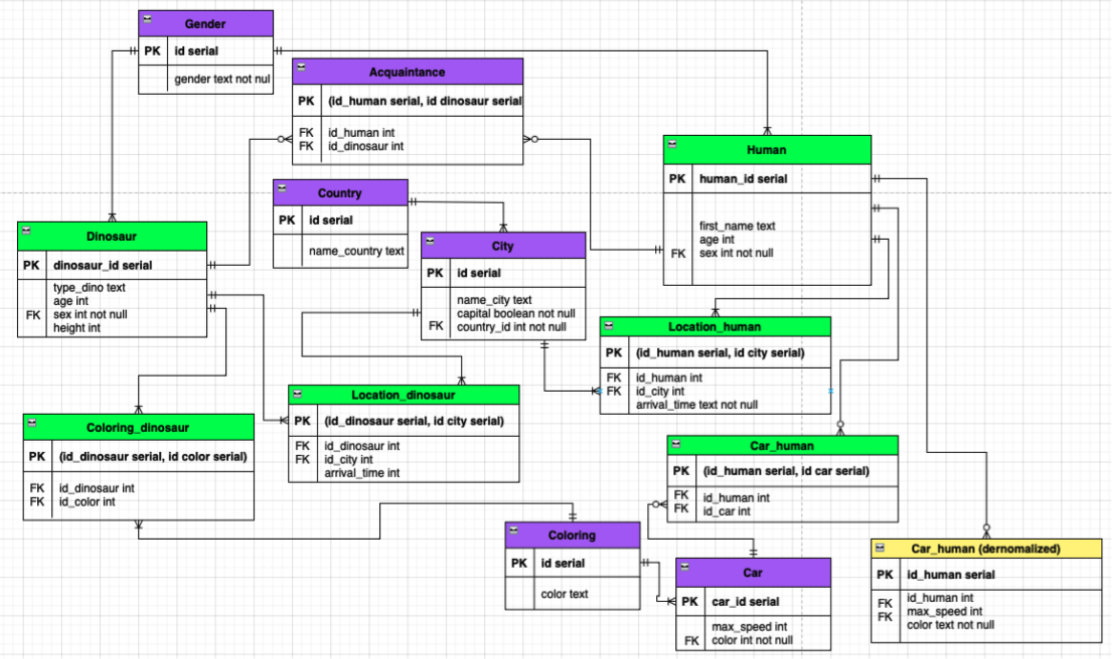
\includegraphics[width=.9\textwidth]{123}